%09.10.2024, lecture 1

\section{Combinatorial approach}

All sets are finite.

\begin{definition}[Hartley, 1928]
    The amount of information in the event $A$ is $\chi(A) = \log \frac{1}{\Pr[A]}$.
\end{definition}

\begin{example}
    Suppose $x \in A$.
    How much information is contained in the fact that $x \in B$?
    \begin{figure}[H]
        \centering
        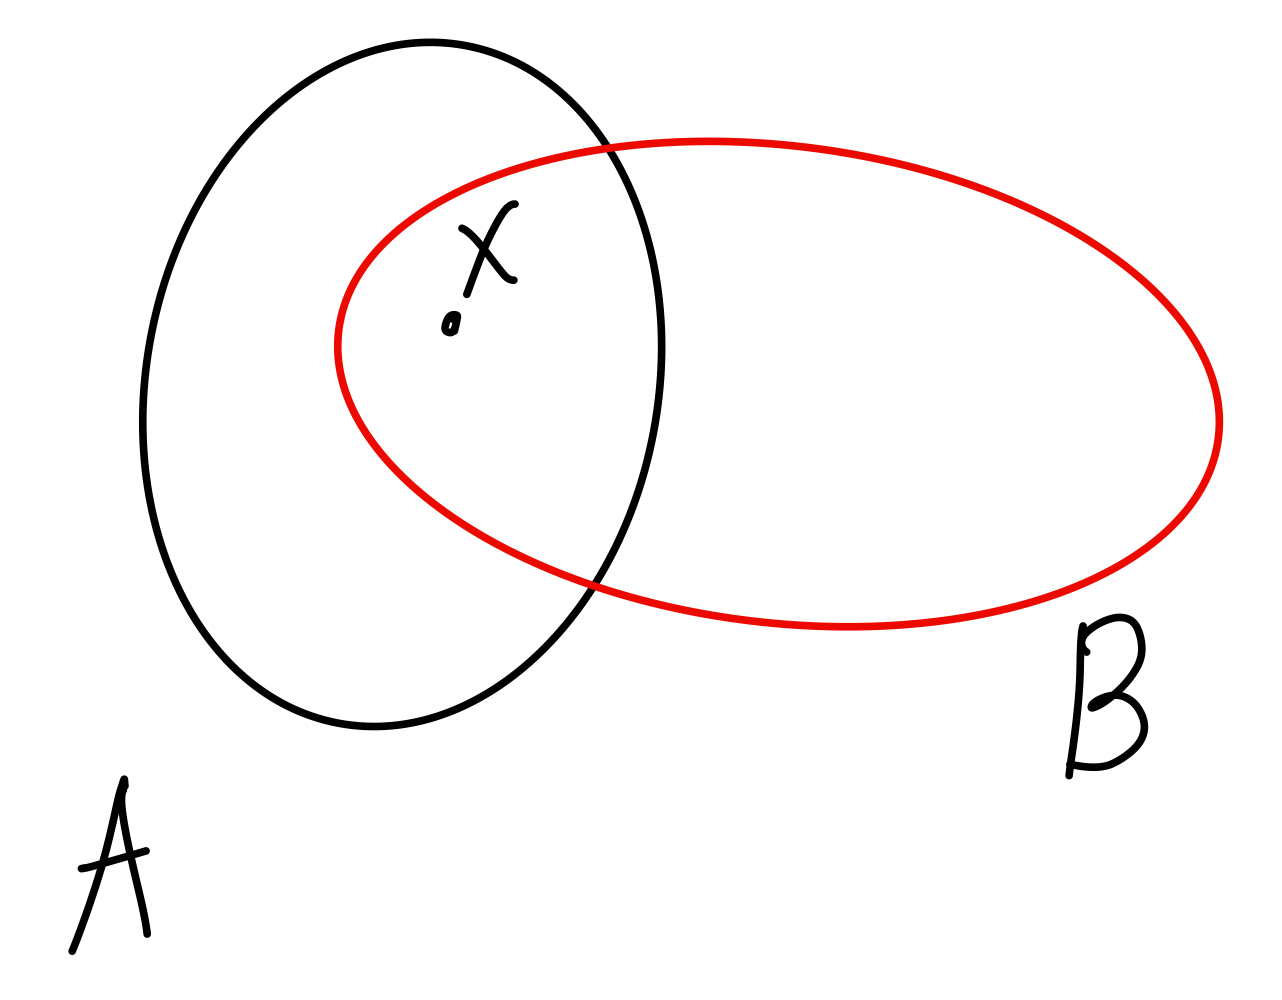
\includegraphics[width=0.3\textwidth]{figures/9268759F-085F-474A-94DD-01FC01C993CA}
        \caption{}
        \label{fig:4cd10f6d-3092-4fca-9f75-1e135943f348}
    \end{figure}

    See \Cref{fig:4cd10f6d-3092-4fca-9f75-1e135943f348}.
    Before we knew that $x \in A$, so we had  $\chi(A)$.
    After we get that $x \in B$, our information became $\chi(A \cap B)$.
    Hence, we got $\chi(A) - \chi(A \cap B)$.
\end{example}

\begin{example}
    If we know that $x \in [100]$, then if we got that $x \divby 2$, then we got  $\log_2 100 - \log_2 50 = 6 - 5 = 1$ bit of information.
\end{example}

\begin{example}
    If we do not know the order of the set $\{a_1, \ldots, a_5\}$, then there is $\log 5!$ of information.
    But if we got that $a_1 > a_2$ or $a_3 > a_4$, then we got $\log (5! - \frac{5!}{4})$.
    Hence, we've learned $\log 5! - \log 90 = \log \frac{4}{3}$.
\end{example}

\begin{definition}
    Let $A \subset \{0, 1\}^* \times \{0, 1\}^*$.
    Denote by $\pi_1(A)$ and $\pi_2(A)$ the projections of the set $A$ onto the first and second coordinates, respectively.
    Then, let $\chi_1(A) = \log |\pi_1(A)|$ and $\chi_2(A) = \log |\pi_2(A)|$.
\end{definition}
\begin{theorem}
    \[\chi(A) \leq \chi_1(A) + \chi_2(A).\]
\end{theorem}
\begin{proof}
    \[
        \log |A| \leq \log |\pi_1(A) \times \pi_2(A)| = \log |\pi_1(A)| + \log |\pi_2(A)| = \chi_1(A) + \chi_2(A). \qedhere
    \]
\end{proof}

\begin{definition}
    The amount of information in the second coordinate of $A \subset \{0, 1\}^* \times \{0, 1\}^*$ given the first coordinate is
    \[\chi_{2 \mid 1}(A) = \log \max_{a \in \pi_1(A)} |\{x \colon (a, x) \in A\}|.\]
\end{definition}

\begin{theorem}
    For any $A \subset \{0, 1\}^* \times \{0, 1\}^*$:
    \[
        \chi(A) \leq \chi_1(A) + \chi_{2 \mid 1}(A).
    \]
\end{theorem}
\begin{proof}
    It is easy to see that
    \[|A| \leq \pi_1(A) \cdot \max_{a \in \pi_1(A)} |\{x \colon (a, x) \in A\}|.\]
    Therefore, theorem is proved.
\end{proof}

\begin{theorem}
    For $A \subset \{0, 1\}^* \times \{0, 1\}^* \times \{0, 1\}^*$:
    \[
        2 \chi(A) \leq \chi_{12}(A) + \chi_{13}(A) + \chi_{23}(A).
    \]
\end{theorem}
\begin{proof}
    See \Cref{fig:b7ba098f-7336-4321-bccd-fc1f6f1419d6}.
    \begin{figure}[H]
        \centering
        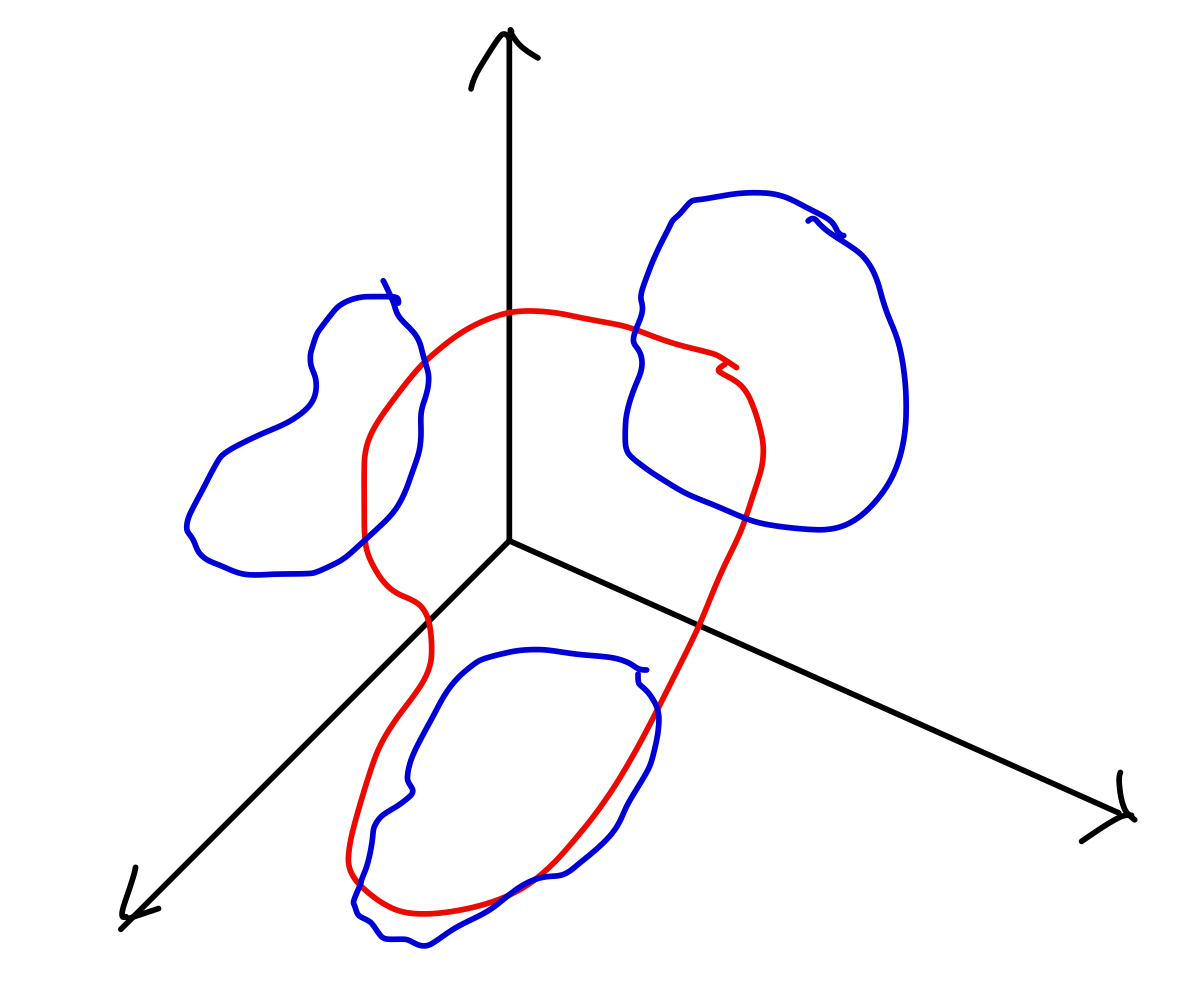
\includegraphics[width=0.3\textwidth]{figures/B7BA098F-7336-4321-BCCD-FC1F6F1419D6}
        \caption{Projections in the three dimensions.}
        \label{fig:b7ba098f-7336-4321-bccd-fc1f6f1419d6}
    \end{figure}

    Will be proved later.
\end{proof}

\begin{corollary}
    The square of the volume of a three-dimensional body does not exceed the product of the areas of its projections onto the coordinate planes.
\end{corollary}

\begin{statement}
    If $f \colon X \to Y$:
    \begin{enumerate}
        \item $f$ is surjective $\then \chi(Y) \leq \chi(X)$;
        \item $f$ is injective $\then \chi(X) \leq \chi(Y)$.
    \end{enumerate}
\end{statement}

\begin{example}
    How many yes/no questions needed to determine a number from $1$ to $N$, if
    a) questions can be asked adaptively.

    b) questions must be written down in advance.
\end{example}
\begin{proof}[Solution]
    a) Obviously $\log N$.
    By simple binary search.

    b) Also $\log N$.
    We should write down the number in binary.

    We can prove the same lower bound.
    If $A$ is a set of possible answers (so we know that answer is in $A$).
    Hence, on each question we can force size of $A$ to decrease at most by 2.

    In terms of information theory we can prove it as follows:
    Let $A = [N]$.
    The set $Q = \{(q_1, \ldots, q_k)\}$ is the set of protocols (answers to the questions).
    Consider $A$ and $Q$ as projections of some set $S$ of all outcomes of the game onto different coordinates.
    Then the following inequalities hold:
    \[
        \chi_Q(S) = \chi(Q) \leq \chi_1(Q) + \chi_2(Q) + \dots + \chi_k(Q) \leq k.
    \]
    And
    \[
        \chi_A(S) = \chi(A) \leq \chi(S) \leq \chi_Q(S) + \underbrace{\chi_{A \mid Q}(S)}_{\text{knows all answers}} \leq k + 0 = k.
    \]
    Thus, we get $\log N = \chi(A) \leq k$.
    Hence, $k = \ceil{\log N}$.
\end{proof}

\begin{example}[Cost of information]
    Let a secret integer be chosen from 1 to $n$ (where $n \geq 2$).
    Any yes/no questions can be asked.
    For a positive answer, we will pay $1$ euro, and for a negative answer ~-- two euros.
    How much it is necessary and sufficient to pay to guess the number?
\end{example}
\begin{proof}[Solution]
    Intuition is simple.
    In case of negative answer we want to get twice more informatino than in case of positive answer.

    Let $A = [n]$ and we are trying to find an answer $x \in A$.
    Let $T$ be a question set (so we are asking: does $x$ in $T$?).
    And let $|T| = \alpha |A|$.
    We want to balance cost of information, hence:

    \begin{align*}
        2 (\chi(A) - \chi(A \cap T)) &= \chi(A) - \chi(A \cap \overline T) &\iff \\
        2 (\log |A| - \log \alpha |A|) &= \log |A| - \log (1 - \alpha) |A| &\iff \\
        -2 \log \alpha &= - \log (1 - \alpha) &\iff \\
        \alpha^2 &= 1 - \alpha & \iff\\
        \alpha &= \frac{-1 + \sqrt 5}{2} \approx 0.618.
    \end{align*}

    Hence, for 1 euro we got $- \log \alpha$ information.
    Hence, we need to pay $- \frac{\log N}{\log \alpha}$ euros.

    In order to construct an algoritheorem we can use rounding.
    But we can do better.
    We will just use numbers from $\R$ in our questions.
    So, the first one would be: does $x$ belong to $[1, \alpha (N - 1)]$.

    In terms of the lower bound.
    We will compare what is lower $\chi(A) - \chi(A \cap T)$ or $\frac{\chi(A) - \chi(A \cap \overline T)}{2}$.
    And adversary will take one that is less.
\end{proof}

\begin{example}
    How many weighing are needed to sort $N$ stones by weight?
    We can take two stones and compare them.
    Find exact answer to this question for $N = 2, 3, 4, 5$.
\end{example}
\begin{proof}[Solution]
    By merge sort we can get $O(N \log N)$ upper bound.

    We can obtain the same lower bound.
    Our protocol is a decision tree with $N!$ leaves, hence the depth is at least $\log N! \sim N \log N$ (Stirling's formula).

    To bound it without Stirling's formula we can use the following trick.
    \[
        \log N! = \log 1 + \log 2 + \dots + \log n \geq \log \frac n 2 + \log \frac n 2 + 1 + \dots + \log n \geq \frac n 2 \log \frac n 2. \qedhere
    \]

    Some exact answers:
    \begin{itemize}
        \item For $N = 2$ we can use only $1$ comparison.
        \item For $N = 3$ we need at least $\ceil{\log 6!} = 3$, and it is easy to make it with $3$.
        \item For $N = 4$ we need at least $5$ comparisons.
        At first sort $3$ previous rocks, after that use $2$ comparisons to insert the last one to the correct position.
        \item For $N = 5$ we need at least $7$ comparisons.
        We can't do the same trick as for $N = 4$.
        \hw
    \end{itemize}

\end{proof}

\begin{example}
    There are 20 visually identical coins, one of which is fake and lighter than the others.
    How to find the fake coin using a balance scale?
    What is the minimum number of weighings needed?

    Now we can compare any two sets of coins.
\end{example}
\begin{proof}[Solution]
    We can split $A$ into $A_1 \sqcup A_2 \sqcup A_3$ and compare $A_1$ and $A_2$.
    Then, we continue wih one of them.
    It gives us the lower bound and the upper of $\ceil{\log_3 |A|}$.
\end{proof}

\begin{example}
    There are $13$ visually identical coins, one of which is fake (with unknown relative weight).
    Can you find the fake coin and determine its relative weight in three weighings?
\end{example}
\begin{proof}[Solution]
    There are 26 possible answers (because we need to find it is lighter or heavier).
    Hence, our lower bound os $\log_3 26 < 3$.
    If the first weighing is $A_1 \lor A_2$ and $A_3 \colon |A_3| \geq 5$, then in case of $A_1 = A_2$ we need to resolve at least 10 outcomes.
    In case $|A_3| \leq 4$, hence $|A_1| + |A_2| \geq 10$ and $|A_1|, |A_2| \geq 5$.
    Then, we also have at least $10$ possible outcomes.
    Hence, it is impossible to solve in three weightings.
\end{proof}

\begin{example}
    There are $15$ visually identical coins, one of which is fake (with unknown relative weight).
    Can you find the fake coin  in three weightings, if you do not need to determine its relative weight?
\end{example}
\begin{proof}[Solution]
    If we found a coin and cannot determine its relative weight, it means we have never weighed it.
    So, for at least remaining 14 coins we will understand their relative weights.
    So there is $14 \cdot 2 + 1$ possible outcomes.
    Hence, the lower bound is $\log_3 29 > 3$.
\end{proof}

\begin{example}
    There are $14$ visually identical coins, one of which is fake (with unknown relative weight).
    Can you find the fake coin  in three weightings, if you do not need to determine its relative weight?
\end{example}
\begin{proof}[Solution]
    Using idea from the previous example we have the lower bound $\log_3 (13 \cdot 2 + 1) \leq 3$.
    \hw
\end{proof}
\begin{example}
    Find one fake coin among 12 in three weighnings, if its relative weight is unknown.
    Hint: use a \"greedy\" strategy, where each weighting provides maximum information.
\end{example}
\begin{proof}[Solution]
\hw
\end{proof}

\begin{application}
    Suppose $N = 1000$.
    Yes/No questions.
    Allowed to lie at most once.
    Trivial upper bound is $21$.
\end{application}
\begin{proof}[Solution]
    Upper bound is \hw. % We can find some number using 10 questions asking binary representation. And then take 5 first questions, and find a set of numbers that satisfies all of them. Hence we can ask whether the number is in this set or not. We can find question in which he lied using 4 more questions.
    At the end, when we know the answer we can check all our previous questions and find one the lie.
    Hence, if we asked $k$ questions, so in the end we know $\log {k + 1} + \log 1000$ bits.
    Hence, $k \geq 10 + \log {k + 1}$, hence $k \geq 14$.
\end{proof}
